\section{Implementation}
\label{sec:Implementation}

%%%%%%%%%%%%%%%%%%%%%%%
% 3. Implementation (describe the details of what you did, possibly divided in sections, one per major subsystems, e.g., navigation, mapping, HRI, task coordination and integration/architectures)
%%%%%%%%%%%%%%%%%%%%%%%

This section describes how the EKF with its three basic steps has been implemented for the faced robot localization problem with a LRF. In subsection \ref{subsec:Prediction} the motion model and the observation model are discussed. The subsections \ref{subsec:Matching} and \ref{subsec:Update} deal with the matching and the update step respectively. The resulting scheme of the implementation is shown in figure \ref{fig:EKF_scheme}. 

\begin{figure}[h]
\centering
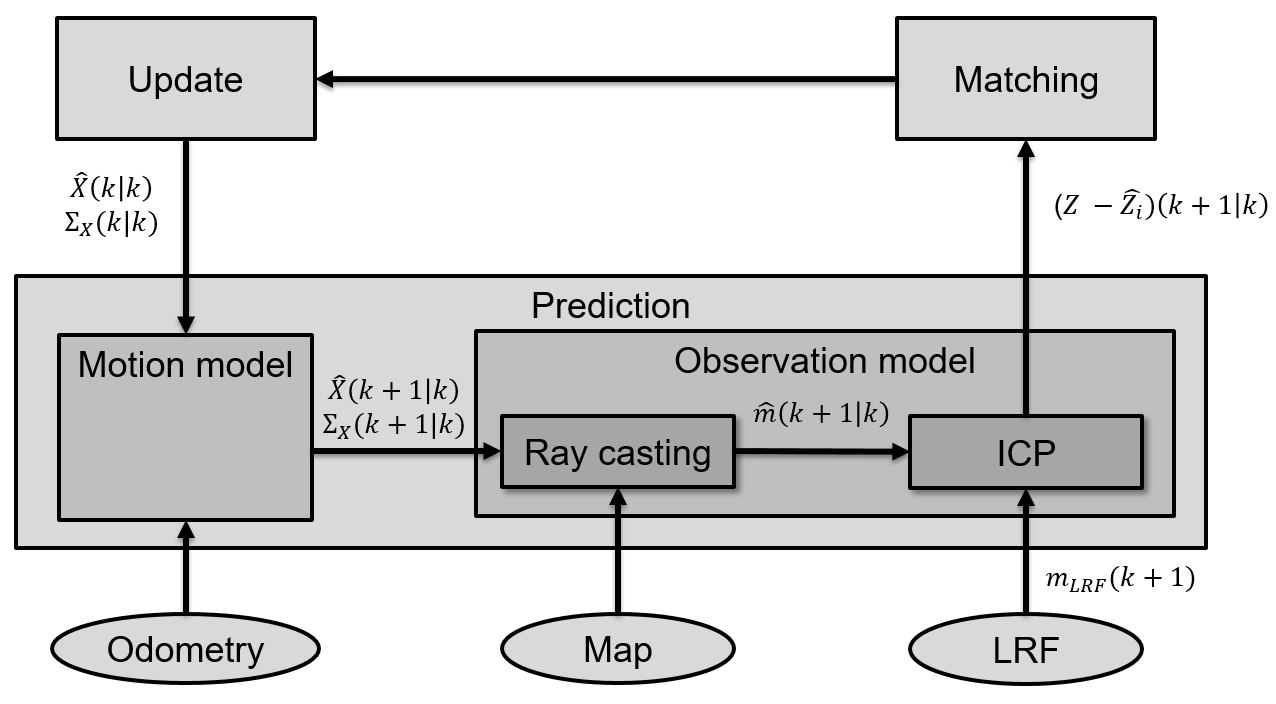
\includegraphics[width=0.45\textwidth]{figures/scheme}
      \caption{Scheme of the implemented EKF}
      \label{fig:EKF_scheme}
\end{figure}

The robot's state $X$ is defined as its current two dimensional pose. The observation $Z$ used for the Extended Kalman filter, like explained in section \ref{subsec:Matching}, also includes variables to describe a pose. 
\begin{align}
X&=\begin{pmatrix}x_s & y_s & \theta_s \end{pmatrix}^T \label{eq:state_def} \\
Z&=\begin{pmatrix}x_{obs} & y_{obs} & \theta_{obs} \end{pmatrix}^T \label{eq:observation_def}\\
V&=Z(k+1)-\hat{Z}(k+1)=\begin{pmatrix} \Delta x_{v} & \Delta y_{v} & \Delta \theta_{v} \end{pmatrix}^T \label{eq:v_def}
\end{align}

With the state and the observation being a 3 by 1 vector, the dimensions of all the variables used in the EKF are defined. Table \ref{tab:Variables_def} lists the used variables with their symbols, dimensions and a short description..
\begin{table}[h]
\centering
\begin{tabular}{>{\centering\arraybackslash}p{1.5cm} >{\centering\arraybackslash}p{1.5cm} >{\small}p{4.5cm}}%{lcc}
\toprule
Symbol & Dimension & Description \\
\midrule
$X$ & 3 x 1 & State vector - Robot pose \\
$V$ & 3 x 1 & ICP observation difference \\
$Z$ & 3 x 1 & Observation \\
$\Sigma$ & 3 x 3 & Robot state covariance  \\
$f$ & 3 x 1 & Motion model function \\
$F$ & 3 x 3 & Motion model Jacobian \\
$Q$ & 3 x 3 & Motion model noise \\
$U$ & 2 x 1 & Motion model input \\
$m^{i}$ & 2 x 1 & Laser beam measurement \\
$h$ & 3 x 1 & Observation model function \\
$H$ & 3 x 3 & Observation model Jacobian \\
$R$ & 3 x 3 & Observation model noise \\
$K$ & 3 x 3 & Kalman gain \\
\bottomrule
\end{tabular}
\caption{Variables and functions used for the EKF}
\label{tab:Variables_def}
\end{table}

\subsection{Prediction}
\label{subsec:Prediction}
The aim of the EKF prediction step is to receive the updated state and covariance and then from there on determine the predicted observation for the next time step $\hat{Z}_i(k+1|k)$. To do so, the motion model predicts the future state in the next time step $\hat{X}(k+1|1)$ and the corresponding covariance matrix $\Sigma_X (k+1|k)$. From there on it is possible for the observation model to obtain the predicted observation $\hat{Z}_i(k+1|k)$. 
The motion and observation model need to be defined by the user depending on the problem and solution approach.
\subsubsection{State Prediction}
\label{subsubsec:State_Prediction}
One of the main ideas of the EKF lies in linearising the motion and measurement model.
For the state prediction, the motion model is decomposed as the noise-free part in  \eqref{eq:state_predict_def} and a random noise component with zero mean in equation \eqref{eq:cov_predict_def}.
\begin{align}
\hat{X}(k+1|k) &= f(\hat{X}(k),~U(k)) \label{eq:state_predict_def} \\
\Sigma_{X}(k+1|k) &= F \Sigma_{X}(k|k) F^{T} + Q(k) \label{eq:cov_predict_def} 
\end{align}
As the considered robot is a three-wheeled vehicle that drives in a planar two dimensional environment, a motion model can be developed for specifically for this case. The Pioneer 3DX is steered by giving different speed commands to the left and right wheel. Therefore, the motion input vector is defined as in \eqref{eq:input}.
\begin{equation}
U=\begin{pmatrix}\omega_{Right} & \omega_{Left} \end{pmatrix}^T \label{eq:input}
\end{equation}
\noindent\begin{minipage}{.53\linewidth}
\centering
\begin{equation}
\beta=\frac{\omega_{Right}-\omega_{Left}}{d} \label{eq:beta}
\end{equation}
\end{minipage}%
\begin{minipage}{.38\linewidth}
\centering
\begin{equation}
R=\frac{\omega_{Left}}{\beta} \label{eq:R}
\end{equation}
\end{minipage}

With the help of $d$, the distance between the robot's driven wheels, and the defined parameters $R$ and $\beta$ in \eqref{eq:beta} respectively \eqref{eq:R}, it is possible to formulate the motion model function in equation \eqref{eq:f_def}.
\begin{equation}
f = \begin{pmatrix} \hat{x}_s(k) + (R+\frac{d}{2})(sin(\hat{\theta}_s+ \beta)-sin(\hat{\theta}_s)) \\ \hat{y}_s(k) + (R+{\frac{d}{2}})(-cos(\hat{\theta}_s+ \beta)+cos(\hat{\theta}_s)) \\ \hat{\theta}_s(k) + \beta\end{pmatrix}
\label{eq:f_def}
\end{equation}

For calculation the predicted state covariance $\Sigma_{X}(k+1|k)$ with equation \eqref{eq:cov_predict_def} the Jacobian $F$ of the motion model function is needed. It can be calculated by derivating $f$ with respect to the state $X$.
\begin{equation}\label{eq:MotionModel}
    \resizebox{0.88\hsize}{!}{%
        $F = \frac{\partial f}{\partial X} = \begin{pmatrix} 1 & 0 & (R+{\frac{d}{2}})(cos(\hat{\theta}_s+ \beta)-cos(\hat{\theta}_s)) \\ 0 & 1 & (R+\frac{d}{2})(sin(\hat{\theta}_s+ \beta)-sin(\hat{\theta}_s)) \\ 0 & 0 & 1\end{pmatrix}$%      
        }
\end{equation}

The Pioneer 3DX robot is able to determine its odometry off the shelf. By using backward differences the next state can also be predicted. With this solution approach the equations for the motion model function $f$ and its Jacobian $F$ can be simplified to equation \eqref{eq:f_simple} and \eqref{eq:F_simple}. 
\begin{align}
f &= \begin{pmatrix} \hat{x}_s(k) + \Delta x_{odom}(k) \\ \hat{y}_s(k) + \Delta y_{odom}(k) \\ \hat{\theta}_s(k) + \Delta \theta_{odom}(k)\end{pmatrix}
\label{eq:f_simple} \\ \nonumber \\
F &= \begin{pmatrix} 1 & 0 & - \Delta y_{odom}(k) \\ 0 & 1 & \Delta x_{odom}(k) \\ 0 & 0 & 1\end{pmatrix} \label{eq:F_simple}
\end{align}
The motion model noise $Q$ represents the trust in the by the motion model predicted state. The in equation \eqref{eq:Q_dynamic} defined noise is implemented with a static and a dynamic component. The static component represents that the robot may even slip while the odometry does not notice any movement. The dynamic component mirrors that the odometry errors accumulate with the amount of movement within a time step.
\begin{equation}
Q = \begin{pmatrix} 1 & 0 & 0 \\ 0 & 1 & 0 \\ 0 & 0 & 1\end{pmatrix} \cdot \begin{pmatrix} q_{x,stat} + q_{x,dyn} |\Delta x_{odom}(k)| \\ q_{y,stat} + q_{y,dyn} |\Delta y_{odom}(k)|  \\ q_{\theta,stat} + q_{\theta,dyn} |\Delta \theta_{odom}(k)| \end{pmatrix}
\label{eq:Q_dynamic}
\end{equation}

\subsubsection{Observation Prediction}
\label{subsubsec:Observation_Prediction}
The observation prediction uses the predicted state from the described state prediction to determine a predicted observation.
It is composed by two parts. The ray casting algorithm and the Iterative Closest Point (ICP) algorithm.

The ray casting enters the pre-acquired map, which is stored as an occupancy grid, at the predicted state $\hat{X}(k+1|k)$ and simulates a laser scan, with the same maximum range, starting angle, ending angle and angle increment as the used laser rangefinder. The algorithm starts at the starting angle and searches for the first occupied grid cell in this direction. It calculates the distance between the predicted state position and the occupied cell and stores it. This is repeated for every laser beam until the ending angle of the real laser is reached. The calculated values $\hat{m}(k+1|k)$ are then handed to the ICP algorithm in the same format as the real laser scan $m_{LRF}(k+1|k)$ .
The idea of the algorithm is shown in figure \ref{fig:Raycasting}. The maximum accuracy is limited by the resolution of this map, which equals $0,05~\frac{m}{pixel}$.
\begin{figure}[h!]
\centering
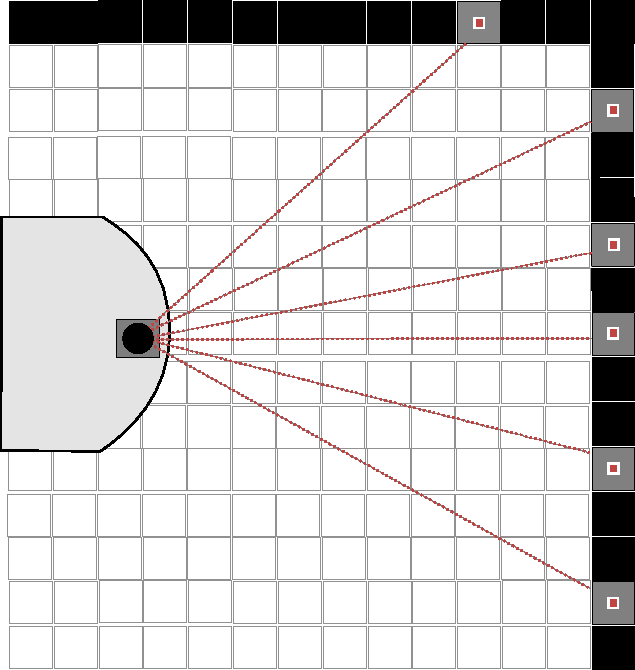
\includegraphics[width=0.3\textwidth]{figures/raycast.pdf}
      \caption{Raycasting}
      \label{fig:Raycasting}
\end{figure}

The Iterative Closes Point algorithm (ICP) to minimize the distance between two clouds of points. One of the point clouds is the reference or target point cloud, which is kept fixed. The other one, the source point cloud, is transformed to best match the reference.
\begin{figure}[h!]
\centering
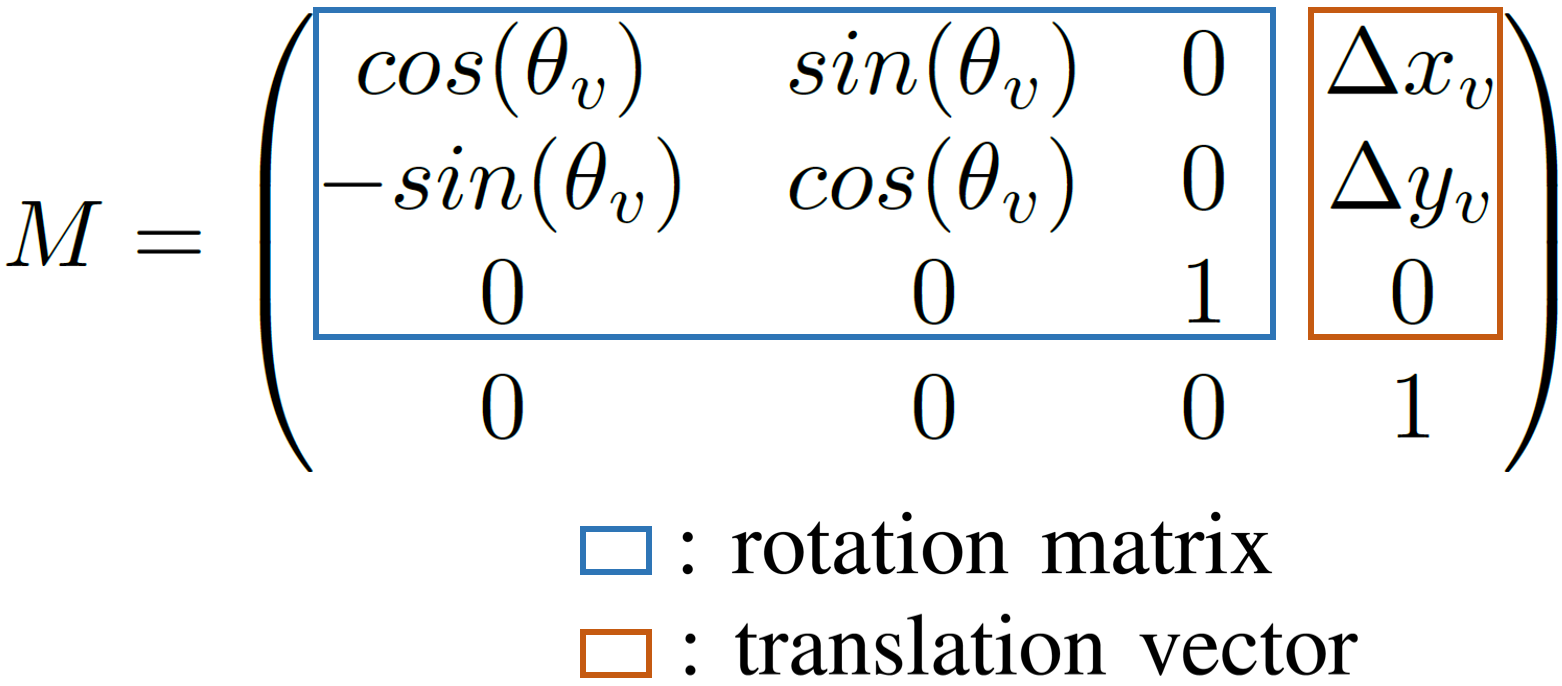
\includegraphics[width=0.35\textwidth]{figures/M}
      %\caption{ICP transformation matrix}
      \label{fig:transformation_matrix}
\end{figure}

The used ICP algorithm is part of the PCL C++ library. If the algorithm converged, it returns a four by four transformation matrix between the two point clouds. The transformation matrix includes a three dimensional rotation matrix and a translation vector. The observation difference vector $V$, defined in equation \eqref{eq:v_def}, between the real observation and the predicted one can be extracted from the ICP transformation matrix. 

\subsection{Matching}
\label{subsec:Matching}
The matching step in the extended Kalman filter generally prevents updates with outliers. In the implemented EKF the matching is also responsible for checking the ICP algorithm quality and for determining the trust into the ICP's result. 

To do so two mismatch conditions have been implemented.
\begin{itemize}
\item ICP did not converge
\item ICP did not match more points than the set threshold of 500 out of 720 points
\end{itemize}
If one of these conditions is fulfilled the next state $\hat{X}(k+1|k+1)$ and and the next covariance $\Sigma_X (k+1|k+1)$ will be set equal to the odometry predicted state $\hat{X}(k+1|k$ calculated with equation \eqref{eq:state_predict_def}, respectively the odometry predicted covariance $\Sigma_{X}(k+1|k)$ of equation \eqref{eq:cov_predict_def}.

\subsection{Update}
\label{subsec:Update}
If none of the mismatching conditions is fulfilled the update step will use the results from the ICP to combine them with the odometry predicted state to make a more precise prediction of the current state and covariance, based on odometry and LRF. 

Because the observation model is based on the ICP, which will give results linear dependent to the predicted state \mbox{$X(k+1|k)$}, the Jacobian of the observation model $H$ results in a \mbox{3 by 3} identity matrix.
\begin{equation}
H = \frac{\partial h}{\partial X} =\begin{pmatrix} 1 & 0 & 0 \\ 0 & 1 & 0 \\ 0 & 0 & 1\end{pmatrix} \label{eq:H_def}
\end{equation}

With $H$ being an identity matrix the formulas for the extended Kalman filter update step can be significantly simplified. The Kalman \mbox{gain $K(k+1)$} can be calculated with only the predicted covariance $\Sigma_{X}(k+1|k)$ and the observation noise \mbox{matrix $R$}. The noise and inaccuracies form the laser rangefinder itself, the ray casting, the mapping and the ICP calculations are summed up in the observation noise matrix $R$. Therefore, the values are much higher than for the laser rangerfinder alone.
\begin{equation}\label{eq:Kalman_def}
    \resizebox{0.89\hsize}{!}{%
        $K(k+1)= \Sigma_{X}(k+1|k)\cdot {(\Sigma_{X}(k+1|k) + R(k+1)})^{-1} $%      
        }
\end{equation}
\begin{equation}
R= \begin{pmatrix} 0.01 & 0 & 0 \\ 0 & 0.01 & 0 \\ 0 & 0 & 0.01\end{pmatrix}\label{R_def}
\end{equation}

The state and covariance update equations are given in \eqref{eq:state_update_def} and \eqref{eq:cov_update_def}. For the state update the observation difference vector $V$, calculated by the ICP algorithm, as well as the Kalman gain $K(k+1)$, are used. The next covariance only depends on the predicted covariance and the Kalman gain.
\begin{align}
& \hat{X}(k+1|k+1) = \hat{X}(k+1|k) + K(k+1)V(k+1) \label{eq:state_update_def} \\
& \Sigma_{X}(k+1|k+1) = (I-K(k+1))\cdot\Sigma_{X}(k+1|k) \label{eq:cov_update_def}
\end{align}


%\subsubsection{Subsubsection Heading Here}
%\label{subsubsec:subsubsection_Tag}
%Subsubsection text here.
